\section{Theorie}
\label{sec:Theorie}
  
  Der Compton-Effekt bezeichnet die Vergrößerung der Wellenlänge von $\gamma$-Strahlung bei der Streuung an einem Elektron.
  
  Bei diesem Versuch wird eine indirekte Methode der Bestimmung der Compton-Wellenlänge mit Hilfe von Röntgenstrahlen durchgeführt. 
  Die Röntgenstrahlen werden an einem Plexiglasquader gestreut und die gestreute Strahlung wird mittels des Transmissionsverhaltens auf ihrer Compton-Wellenlänge untersucht.\\
  Die Streustrahlung an Materie setzt sich aus die klassische inelastische Streuung (kohähenten Streuung) und die elatische frequenzverschobene Streuung (inkohänente oder Compton Streuung), bei der gibt es Energie- und Impulsaustausch zwischen einem Photon und einem um den Winklel $\theta$ gestreuten Elektron.
  Die Zunahme der Wellenlänge $\Delta \lambda$ lässt sich mittels
\begin{equation}
  \Delta \lambda= \frac{h}{m_e \cdot c}(1-\cos \theta)
\end{equation} berechnen.
  Die Formel für die Compton-Wellenlänge des Elektrons lautet \(\lambda_c =\frac{h}{m_e \cdot c}\).
  \paragraph{}
   Für die Erzeugung von Röntgenstrahlen mit der Röntgenröhre werden die elektromagnetische Wellen, die bei der Abbremsung der von einer Glühkathode auf eine Anode schnell beschleunigten Elektronen entstehen, verwendet.
  Bei Auftreten auf die Anode entsteht eine Röntgenstrahlung, die sich aus der kontinuierlichen Bremsspektrum und der charakteristischen Röntgenstrahlung überlagert ist.

\begin{figure}[H]
    \centering
    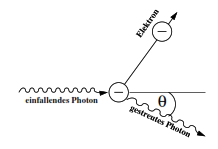
\includegraphics{Compton-Effekt.png}
    \caption{Compton-Effekt.}
    \label{fig:Compton-Effekt}
  \end{figure}
   Bei der Abbremsung eines Elektrons entsteht ein Bremsspektrum und ein Photon, auf welches der Energieverlust (ein Teil oder die gesamte kinetische Energie) des abgebremsten Elektrons übergetragen wird.
Das Bremsspektrum setzt sich aus 2 Teilspektren zusammen: kontinuierliches und charakteristisches Spektrum. 
Das charakteristisches Spektrum entsteht, wenn das Anodematerial ionisiert wird, indem ein Elektron in die innere Schale durch die Aussendung eines Röntgenquants zurückfällt. 
Die Energiedifferenzen entsprechen der Energie des Röntgenquants und des Linienspektrums der (für das jeweilige Anodematerial) charakteristischen Röntgenstrahlung.

 Durch Aluminium werden für die Bestimmung der Compton-Wellenlänge die Transmission und Absorption von Röntgenstrahlung ausgenutzt. 
Die Transmission des Stoffes nimmt mit zunehmender Wellenlänge ab.
Für die Absorption entsteht das Lambert-Beer'sche Gesetz
\begin{equation}
  I = I_0 e^{-\mu d}
\end{equation}
wobei: $I_0$ bzw. $I$ ist einfallende und verschobene Intensität.\\
       Der Absorptionskoeffizient ist \(\mu = \mu_\text{Paar}+ \mu_\text{Photo}+\mu_\text{Com}\), wobei die Absorptionskoeffiziente $\mu_\text{Paar}$, $\mu_\text{Photo}$, $\mu_\text{Com}$ für Paarbildung, Photoeffekt und Comptoneffekt stehen.

\paragraph{}
Die Energie und die Wellenlänge $\lambda$ der Röntgenstrahlung können durch die Bragg’sche Reflexion auf ein 3-D Gitter annalysiert werden.
Die Röntgenstrahlen reflektieren konstruktiv vom Gitter nur bei bestimmte Auftriffwinkeln (Glanzwinkeln) $\alpha$.
 \begin{figure}[H]
    \centering
    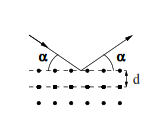
\includegraphics{Gitterkonstanten.png}
    \caption{Die Bragg’sche Reflexion.}
    \label{fig:Gitterkonstanten}
  \end{figure}
Daher lautet die Bragg’sche Bedingung:
\begin{equation}
  2d \sin \alpha = n \lambda 
\end{equation}
mit der Wellenlänge $\lambda$, Beugungsordnung $n$ und Gitterkonstanten $d$ (\(d_\text{LiF}=201,4\, \mathrm{pm} \)). 
\cite{AL}
\newpage
